\begin{wrapfigure}[10]{r}{0.28\textwidth}
\small
\renewcommand*{\arraystretch}{0.75}

\def\CircFix{(135:0.707cm) circle (1.5cm)}
\def\CircProd{(45:0.707cm) circle (1.5cm)}
\def\CircIsorec{(-45:0.707cm) circle (1.5cm)}
\def\CircSum{(-135:0.707cm) circle (1.5cm)}

\definecolor{FixColor}{HTML}{FF9966}
\definecolor{ProdColor}{HTML}{66CCFF}
\definecolor{SumColor}{HTML}{FFFF66}
\definecolor{IsorecColor}{HTML}{FF6699}

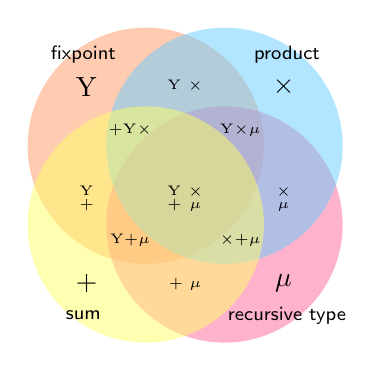
\begin{tikzpicture}
    \begin{scope}[shift={(0cm,-0cm)}, fill opacity=0.50]
        \fill[FixColor] \CircFix;
        \fill[IsorecColor] \CircIsorec;
        \fill[ProdColor] \CircProd;
        \fill[SumColor] \CircSum;
%       \draw \CircFix;
%       \draw \CircIsorec;
%       \draw \CircProd;
%       \draw \CircSum;
    \end{scope}

    \node at (0: 0) {%
        \begin{minipage}{1cm}\tiny
        \[\begin{array}{@{}c@{\ }c@{}}
            \mathrm{Y} & \times\\ + & \mu
        \end{array}\]
        \end{minipage}
    };
    \node at (-180: 1.25cm) {%
        \begin{minipage}{1cm}\tiny
        \[\begin{array}{@{}c@{}}
            \mathrm{Y}\\ +
        \end{array}\]
        \end{minipage}
    };
    \node at (0: 1.25cm) {%
        \begin{minipage}{1cm}\tiny
        \[\begin{array}{@{}c@{}}
            \times\\ \mu
        \end{array}\]
        \end{minipage}
    };
    \node at (90: 1.26cm) {\tiny$\mathrm{Y}\ \times$};
    \node at (-90: 1.26cm) {\tiny$+\ \mu$};
    \node at (135: 1.768cm) {$\mathrm{Y}$};
    \node at (-135: 1.768cm) {$+$};
    \node at (45: 1.768cm) {$\times$};
    \node at (-45: 1.768cm) {$\mu$};
    \node at (45: 0.988cm) {\tiny$\mathrm{Y}$$\times$$\mu$};
    \node at (-45: 0.988cm) {\tiny$\times$$+$$\mu$};
    \node at (-135: 0.988cm) {\tiny$\mathrm{Y}$$+$$\mu$};
    \node at (135: 0.988cm) {\tiny$+$$\mathrm{Y}$$\times$};
    
    \node at (128: 2.1cm) {\scriptsize\sf fixpoint};
    \node at (52: 2.1cm) {\scriptsize\sf product};
    \node at (-52: 2.1cm) {\scriptsize\sf recursive type};
    \node at (-128: 2.1cm) {\scriptsize\sf sum};

\end{tikzpicture}
\end{wrapfigure}